\documentclass[11pt]{article}
\usepackage[margin=1in]{geometry}
\usepackage{amsmath}
\usepackage{booktabs}
\usepackage{caption}
\usepackage{float}
\usepackage{graphicx}
\usepackage{url}
\usepackage{hyperref}
\usepackage{longtable}
\usepackage{siunitx}
\usepackage{xcolor}
\usepackage{enumitem}
\usepackage{array}

\hypersetup{
  colorlinks=true,
  linkcolor=blue!50!black,
  citecolor=blue!50!black,
  urlcolor=blue!50!black
}
\setlist[itemize]{leftmargin=1.35em}
\setlist[enumerate]{leftmargin=1.35em}
\sisetup{round-mode=places,round-precision=3}
\newcolumntype{L}[1]{>{\raggedright\arraybackslash}p{#1}}

\title{Predictive Evaluation Competition: Methods Tried, Hosted Results, and Final Selection}
\author{Competition Technical Report}
\date{June 2026}

\begin{document}
\maketitle

\begin{abstract}
This report summarizes the submission cycle for the Codabench Predictive Evaluation Competition \cite{codabench_competition}. The competition ranks submissions by hosted negative log-loss, with AUC-ROC as a secondary diagnostic metric. Across 94 parsed hosted rows (92 finished scored rows), the best rounded hosted score improved to -0.57. The selected final submission is \path{submission_anchor_fam_b60_debias.zip}, with hosted score -0.57, approximate log-loss 0.57, and competition-reported AUC-ROC 0.73. The main empirical conclusion is that compact domain-prior models were the safest no-label baseline, but the successful break below 0.60 log-loss came from using the platform's random revealed labels as an unbiased hidden-category base-rate anchor.
\end{abstract}

\section{Executive Summary}
This is a competition submission report, not a course-project writeup. It is written around hosted Codabench evidence and the final ZIP intended for publication in the Predictive Evaluation Competition.

The selected submission is \path{submission_anchor_fam_b60_debias.zip}. Its hosted negative log-loss was -0.57, which corresponds to ordinary log-loss about 0.57. The competition interface also reported AUC-ROC 0.73; the local \path{eval_finals.txt} file records the hosted score and submission metadata.

The search first plateaued around \(-0.62\). Compact domain-prior submissions transferred better than AUC stacks, tree blends, forecast ensembles, item-memory models, and hierarchical OOD extensions because they made fewer public-benchmark-specific claims. The extra day changed the diagnosis: the best remaining signal was not another public-data feature, but the random revealed labels supplied by the hosted runtime. The final model estimates the hidden category base rate from those labels and adds a moderate family-aware subject correction.

The original target was hosted log-loss below 0.60, equivalent to displayed negative log-loss above -0.60. The final selected anchor reached that target. The result does not mean local high-AUC evidence was trustworthy; it means the submission finally used hidden-run information in a calibrated way.

\section{Problem Setup And Metric}
The task is amortized prediction of subject-item correctness. At runtime, the submitted \path{model.py} receives visible benchmark, condition, subject content, item content, and a small set of previously revealed labels. It must return \(p_i=\Pr(y_i=1)\) for each hidden row \cite{predictive_asn,codabench_competition}.

The primary metric is negative log-loss:
\[
  \frac{1}{n} \sum_{i=1}^n
  \left[
    y_i\log(p_i)+(1-y_i)\log(1-p_i)
  \right].
\]
This is a negative mean log-likelihood, bounded above by zero, so higher leaderboard values are better. A score of -0.57 is approximately log-loss 0.57. AUC-ROC is secondary: AUC measures ranking, while log-loss also penalizes the absolute probability scale.

The hosted hidden-evaluation setup is central to the result. Public training data came from Measurement DB \cite{measurement_db}, but hidden test items were served only through the runtime. The starter-kit notes state that hidden test items come from benchmarks not present in public training \cite{predictive_asn}. Exact item memory and public benchmark-specific priors were therefore structurally risky.

\section{Data And Hidden-Evaluation Constraints}
The hidden evaluation sampled 5000 items per submission, stratified by organizer data category. The category field was not passed to the predictor. If a submission did not include \path{labeling.py}, the platform revealed a random sample under the same category budget. If a policy was present, the platform used acquisition scores subject to the hidden category budget.

This made two constraints binding. First, public row holdout was too optimistic because benchmark, subject, condition, and sometimes item overlap remained. Second, active labeling could easily bias the revealed sample. Random labels are noisy, but for base-rate estimation they are valuable because they are approximately unbiased for the hidden category.

\section{Methods Tried}
\subsection{Notation And Shared Calibration}
Let \(s\) denote a subject, \(i\) an item, and \(y_{s,i}\in\{0,1\}\) the correctness label. Every submitted method produced a probability \(p_{s,i}\), clipped to \([\epsilon,1-\epsilon]\) to avoid infinite log-loss. Many estimates used shrinkage:
\[
  \operatorname{shrink}(\bar y_g,n_g;c,\tau)
  =
  \frac{n_g\bar y_g+\tau c}{n_g+\tau},
\]
where \(g\) is a group, \(c\) is a base rate, \(n_g\) is support, and \(\tau\) controls pullback toward \(c\). Several models also used temperature-style calibration:
\[
  p'=\sigma\left(\alpha+\beta\,\operatorname{logit}(p)\right),
\]
where \(\beta<1\) cools the probability spread and \(\beta>1\) sharpens it.

\subsection{Global Centers And Subject Priors}
The simplest candidates predicted a constant:
\[
  p_{s,i}=c.
\]
Subject-prior variants added a shrunk visible-subject ability estimate:
\[
  \hat p_s=\frac{n_s\bar y_s+\tau_s c}{n_s+\tau_s},
  \qquad
  p_{s,i}=(1-\lambda_s)c+\lambda_s\hat p_s,
  \qquad
  \lambda_s=\frac{n_s}{n_s+\tau_s}.
\]
Alias matching connected visible subject descriptions to public subject records. These variants were useful calibration baselines, generally scoring around -0.63 to -0.66, but subject priors alone did not identify hidden benchmark difficulty.

\subsection{Benchmark, Condition, And Engineered Priors}
Early engineered variants added public benchmark and condition means:
\[
  p_{s,i}=c+a_s+b_{\mathrm{bench}(i)}+q_{\mathrm{cond}(i)}.
\]
The terms were shrunk toward zero. This improved public-slice validation but had poor hidden-transfer logic: benchmarks not present in public training cannot be recognized by exact public benchmark means. These features therefore became fallback calibration signals rather than final decision rules.

\subsection{Semantic And Text Difficulty Models}
Semantic/text models attempted to infer item difficulty from visible item content and subject descriptors:
\[
  z_{s,i}
  =
  \beta_0+\beta_s^\top\phi_s(x_s)
  +\beta_i^\top\phi_i(x_i)
  +\beta_{si}^\top\phi_{si}(x_s,x_i),
  \qquad
  p^{\mathrm{text}}_{s,i}=\sigma(z_{s,i}).
\]
Feature maps \(\phi\) represented domain keywords, task-type cues, difficulty markers, subject-family indicators, and semantic similarity features. The text score was usually blended with a conservative prior:
\[
  p_{s,i}=(1-\eta)p^{\mathrm{prior}}_{s,i}+\eta p^{\mathrm{text}}_{s,i}.
\]
The failure mode was calibration. Text features sometimes ranked public rows well, but the absolute probability assigned to unseen hidden benchmark families was unstable.

\subsection{Adaptive Labeling Attempts}
The competition permits a small number of labels to be revealed before full prediction. Acquisition policies assigned a score \(r_{s,i}\), such as uncertainty sampling
\[
  r_{s,i}=-|p_{s,i}-0.5|,
\]
or coverage sampling over predicted domains. After labels were revealed, simple adjustment models used
\[
  \Delta_L=\rho(\bar y_L-\bar p_L),
  \qquad
  p^L_{s,i}=\operatorname{clip}(p_{s,i}+\Delta_L,\epsilon,1-\epsilon).
\]
Hosted results did not support aggressive acquisition. A key later lesson is that omitting \path{labeling.py} was beneficial for the final anchor because the platform-random labels preserved an unbiased base-rate estimate.

\subsection{Item Memory And Exact Lookup}
Item-memory models treated normalized public item text as a key:
\[
  \hat p_i
  =
  \frac{n_i\bar y_i+\tau_i p^{\mathrm{fallback}}_{s,i}}{n_i+\tau_i}.
\]
This looked strong under row holdout because public validation rows shared item text with training rows. Under benchmark-family holdout, item coverage was effectively zero, matching the hidden setup. Hosted item-memory variants stayed near -0.63 to -0.64, confirming that exact public item memory did not transfer.

\subsection{AUC Stacks And Pairwise Rankers}
AUC-focused submissions combined component predictors with a logit opinion pool:
\[
  p_{s,i}
  =
  \sigma\left(
    \alpha+\gamma\sum_m w_m\,\operatorname{logit}(p^m_{s,i})
  \right),
  \qquad
  w_m\ge 0.
\]
The scale \(\gamma\) controlled sharpness. Higher sharpness often improved local ranking metrics but increased hidden log-loss risk. Pairwise rankers estimated latent utilities
\[
  \Pr(y_a>y_b)=\sigma(u_a-u_b),
\]
then converted ranks to probabilities. These models were aligned with AUC, not with calibrated log-loss. Hosted AUC/rank variants scored roughly -0.64 to -0.71.

\subsection{Tree Models And Forecast Ensembles}
Tree models used structured subject, domain, text, public-prior, and interaction features. Forecast ensembles then pooled model outputs:
\[
  z_{s,i}=\alpha+\sum_m w_m\,\operatorname{logit}(p^m_{s,i}),
  \qquad
  p_{s,i}=\sigma(z_{s,i}/T).
\]
On public-proxy validation, some forecast optimizers produced log-loss near 0.34 and AUC above 0.928. Hosted results did not transfer, landing around -0.63 to -0.67. The likely cause was overfitting public benchmark and item structure, followed by overconfident probabilities on shifted hidden families.

\subsection{Compact Domain Priors}
The most stable pre-anchor family used broad subject and item-domain signals. Item text was mapped into coarse indicators \(D_k(i)\), and each domain effect was shrunk:
\[
  \delta_k=\frac{n_k}{n_k+\tau_d}(\bar y_k-c),
  \qquad
  d(i)=\sum_k D_k(i)\delta_k.
\]
Subject ability was similarly shrunk:
\[
  a_s=\frac{n_s}{n_s+\tau_s}(\bar y_s-c).
\]
The compact prediction was
\[
  p_{s,i}=\operatorname{clip}\left(c+w_a a_s+w_d d(i),\epsilon,1-\epsilon\right).
\]
This family avoided exact item lookup, public benchmark lookup, and high-variance interactions. Multiple compact domain-prior variants reached the early -0.62 plateau, and the final anchor retained this compact formula as the no-label fallback.

\subsection{Hierarchical OOD Extensions}
Hierarchical OOD variants added subject-domain interactions and conservative revealed-label corrections:
\[
  p_{s,i}
  =
  \operatorname{clip}\left(c+a_s+d(i)+h_{s,d(i)}+\ell_L,\epsilon,1-\epsilon\right),
\]
with
\[
  h_{s,d}
  =
  \frac{n_{s,d}}{n_{s,d}+\tau_h}
  \left(\bar y_{s,d}-c-a_s-d\right).
\]
Cold benchmark-family validation suggested improvement, but hosted results ranged from -0.63 to -0.68. The additional interactions likely added enough variance to hurt log-loss on the hidden sample.

\subsection{Final Domain Micro-Sweeps}
After high-complexity methods degraded, calibration-center sweeps tested whether the hidden base rate was simply lower or higher than 0.60:
\[
  p_{s,i}(c,\lambda)
  =
  \operatorname{clip}\left(c+\lambda(w_a a_s+w_d d(i)),\epsilon,1-\epsilon\right).
\]
Centers from 0.550 to 0.630 and several cooling strengths were submitted. None beat the compact -0.62 plateau. That result made a single global-center correction unlikely to be sufficient.

\subsection{Revealed-Label Anchoring}
The final successful family used random revealed labels as a hidden-run base-rate estimator. For a target row \(i\), the model constructed a hierarchy of grouping keys:
\[
  \mathcal{G}(i)=
  [
    \mathrm{pooled},
    \mathrm{family}(i),
    \mathrm{signature}(i),
    \mathrm{benchmark}(i),
    (\mathrm{benchmark}(i),\mathrm{condition}(i))
  ].
\]
The family and signature levels are coarse groupings derived from visible metadata and text. The benchmark and condition levels are populated only from labels revealed during the hosted run.

For each group \(g\), revealed labels define a Laplace-smoothed rate in logit space:
\[
  m_g=\frac{s_g+\alpha}{n_g+2\alpha},
  \qquad
  \ell_g=\operatorname{logit}(m_g).
\]
Child logits are shrunk toward parent logits:
\[
  \tilde\ell_g
  =
  w_g\ell_g+(1-w_g)\tilde\ell_{\mathrm{parent}(g)},
  \qquad
  w_g=\frac{n_g}{n_g+\tau},
\]
with \(\alpha=1\) and \(\tau=4\) in the selected variant. This makes the prediction close to the hidden category's observed base rate while limiting overconfidence from small samples.

The model then adds a family-aware subject correction. Public data estimate
\[
  o_{s,f}
  =
  \operatorname{clip}\left(
    \operatorname{logit}(\hat p_{s,f})
    -
    \operatorname{logit}(\hat p_f),
    -c_o,c_o
  \right).
\]
The selected debiased variant subtracts the mean subject offset in the revealed sample and adds the target subject's offset:
\[
  z_{s,i}
  =
  \tilde\ell_{g^*(i)}-\beta\bar o_L+\beta o_{s,f(i)},
  \qquad
  p_{s,i}=\sigma(z_{s,i}),
\]
where \(\beta=0.60\). Offline simulation of the exact runtime with random revealed labels selected the family-aware debiased configuration, and hosted evaluation confirmed it: \path{submission_anchor_fam_b60_debias.zip} scored -0.57. Nearby anchor variants also showed the risk of over-adjustment, ranging from -0.60 to -0.82.

\section{Hosted Results}
\begin{table}[H]
\centering
\small
\caption{Final selected hosted submission.}
\label{tab:selected}
\setlength{\tabcolsep}{5pt}
\begin{tabular}{L{0.28\linewidth}L{0.62\linewidth}}
\toprule
Field & Value \\
\midrule
ZIP & \path{submission_anchor_fam_b60_debias.zip} \\
Hosted submitted time & 2026-06-06 07:28 \\
Hosted negative log-loss & -0.57 \\
Approximate log-loss & 0.57 \\
AUC-ROC & 0.73 (competition reported) \\
Runtime family & Revealed-label anchored base-rate model with compact domain-prior fallback \\
\bottomrule
\end{tabular}
\end{table}


\begin{table}[H]
\centering
\small
\caption{Hosted negative log-loss by method family. Scores are leaderboard values; higher is better.}
\label{tab:family-summary}
\setlength{\tabcolsep}{4pt}
\begin{tabular}{L{0.25\linewidth}rrrL{0.35\linewidth}}
\toprule
Family & Rows & Best score & Median score & Best ZIP \\
\midrule
Compact domain prior & 17 & -0.62 & -0.63 & \path{submission_domain_prior_hidden_cent.zip} \\
Final domain micro-sweep & 8 & -0.62 & -0.64 & \path{submission_domain_live_mid610.zip} \\
Alias/scaled priors & 15 & -0.63 & -0.63 & \path{submission_alias_light.zip} \\
External/domain prior & 4 & -0.63 & -0.63 & \path{submission_external_domain_mid600.zip} \\
Forecast ensemble & 5 & -0.63 & -0.63 & \path{submission_forecast_robust_logloss_.zip} \\
Hierarchical OOD & 5 & -0.63 & -0.66 & \path{submission_hier_ood_center600.zip} \\
Item memory & 2 & -0.63 & -0.64 & \path{submission_item_memory_rank.zip} \\
AUC/rank stack & 6 & -0.64 & -0.65 & \path{submission_auc_stack_item_push_labe.zip} \\
Baseline/calibration & 7 & -0.64 & -0.66 & \path{submission_calibrated_constant.zip} \\
Other & 3 & -0.64 & -0.65 & \path{submission_subject_balanced.zip} \\
Tree blend & 3 & -0.64 & -0.64 & \path{submission_tree_blend_maxauc_labeli.zip} \\
OOD gated & 2 & -0.65 & -0.66 & \path{submission_ood_gated.zip} \\
Semantic/text & 3 & -0.65 & -0.65 & \path{submission_semantic_labeling.zip} \\
\bottomrule
\end{tabular}
\end{table}


\begin{table}[H]
\centering
\scriptsize
\caption{All finished submissions tied for the best rounded hosted score in \texttt{eval\_finals.txt}.}
\label{tab:best-rows}
\setlength{\tabcolsep}{3pt}
\begin{tabular}{rL{0.17\linewidth}rL{0.18\linewidth}L{0.38\linewidth}}
\toprule
ID & Date & Score & Family & ZIP \\
\midrule
777007 & 2026-06-02 22:26 & -0.62 & Compact domain prior & \path{submission_domain_prior_hidden_cent.zip} \\
777016 & 2026-06-02 22:28 & -0.62 & Compact domain prior & \path{submission_domain_prior_publiccal.zip} \\
777017 & 2026-06-02 22:28 & -0.62 & Compact domain prior & \path{submission_domain_prior_sweep_loglo.zip} \\
777204 & 2026-06-03 00:25 & -0.62 & Compact domain prior & \path{submission_domain_live_sweep_s085.zip} \\
777209 & 2026-06-03 00:26 & -0.62 & Compact domain prior & \path{submission_domain_live_mid600.zip} \\
777210 & 2026-06-03 00:26 & -0.62 & Compact domain prior & \path{submission_domain_live_mid620.zip} \\
777211 & 2026-06-03 00:26 & -0.62 & Compact domain prior & \path{submission_domain_live_mid640.zip} \\
777214 & 2026-06-03 00:27 & -0.62 & Compact domain prior & \path{submission_domain_live_pub_s115.zip} \\
781993 & 2026-06-05 15:45 & -0.62 & Final domain micro-sweep & \path{submission_domain_live_mid610.zip} \\
\bottomrule
\end{tabular}
\end{table}


Figure~\ref{fig:hosted-time} plots finished hosted scores by submission order. Figure~\ref{fig:best-family} summarizes the best score by method family. Figure~\ref{fig:narrative} shows the search narrative: compact domain-prior candidates established the -0.62 plateau, higher-complexity candidates mostly failed to improve it, and revealed-label anchoring produced the -0.57 best row.

\begin{figure}[H]
  \centering
  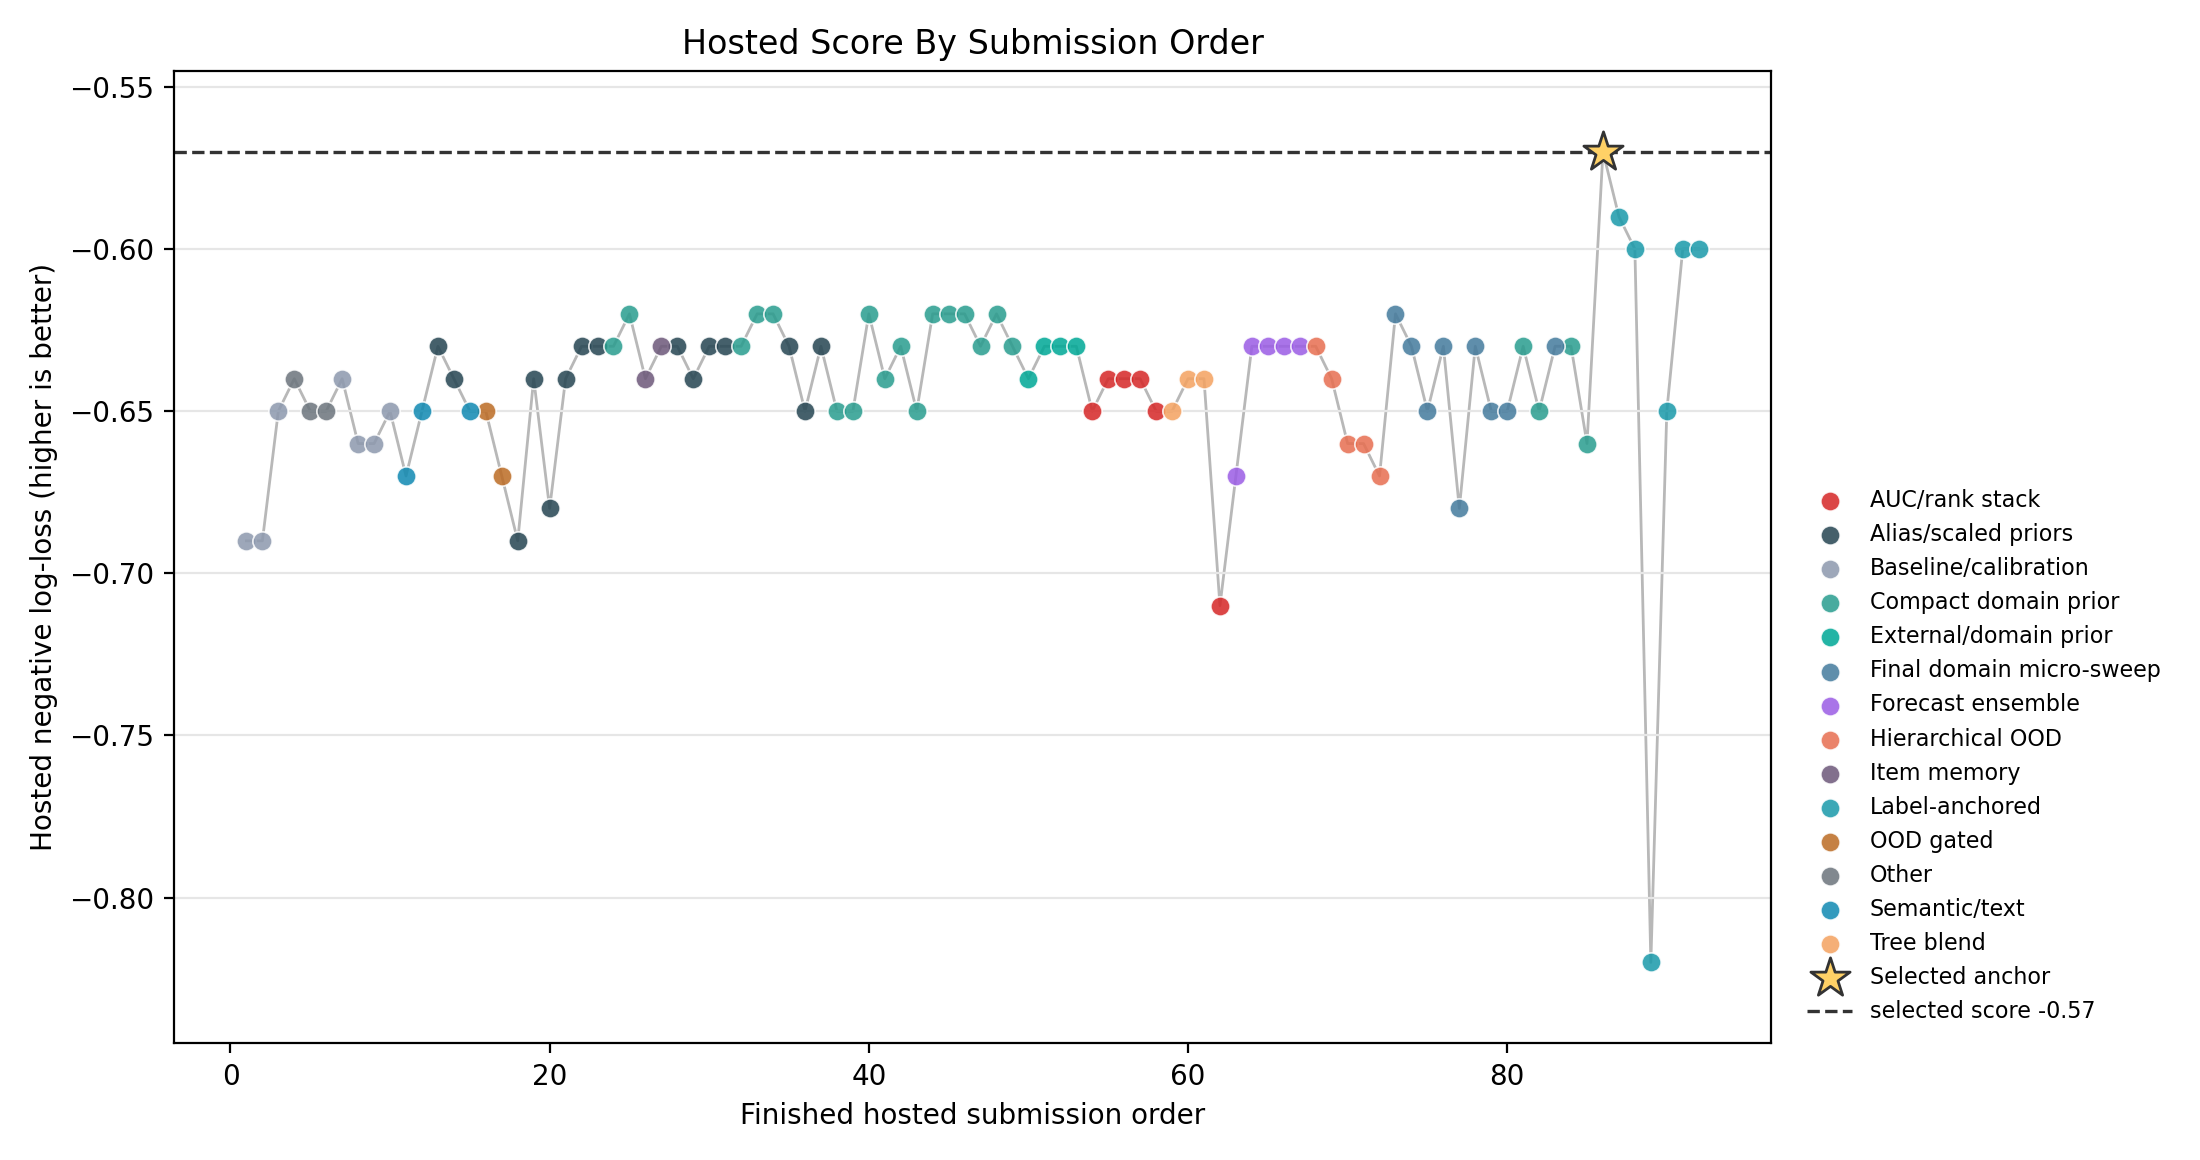
\includegraphics[width=\linewidth]{figures/hosted_scores_over_time.png}
  \caption{Hosted negative log-loss by finished submission order, colored by method family.}
  \label{fig:hosted-time}
\end{figure}

\begin{figure}[H]
  \centering
  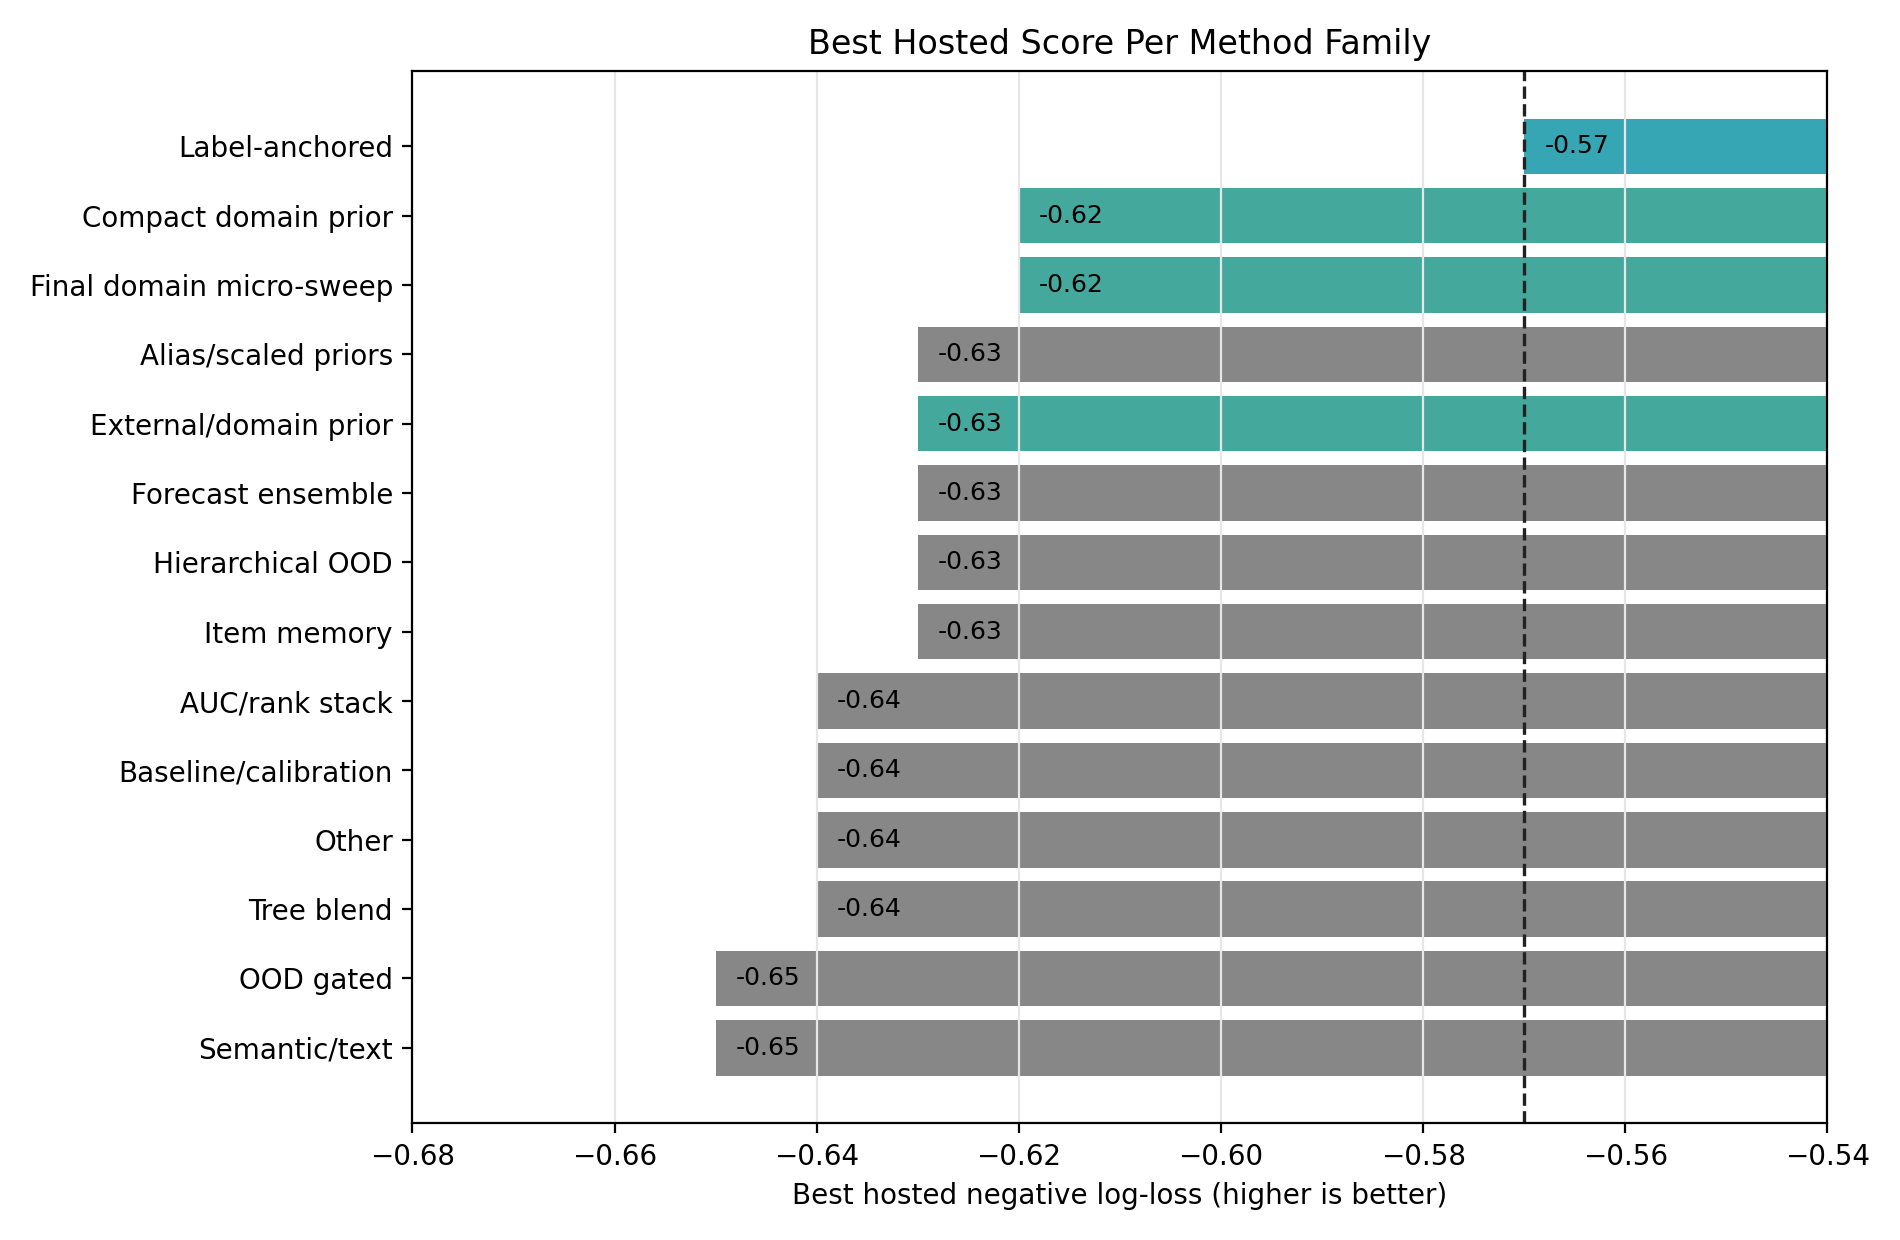
\includegraphics[width=0.92\linewidth]{figures/best_by_family.png}
  \caption{Best rounded hosted score per method family. The dashed line marks the selected score.}
  \label{fig:best-family}
\end{figure}

\begin{figure}[H]
  \centering
  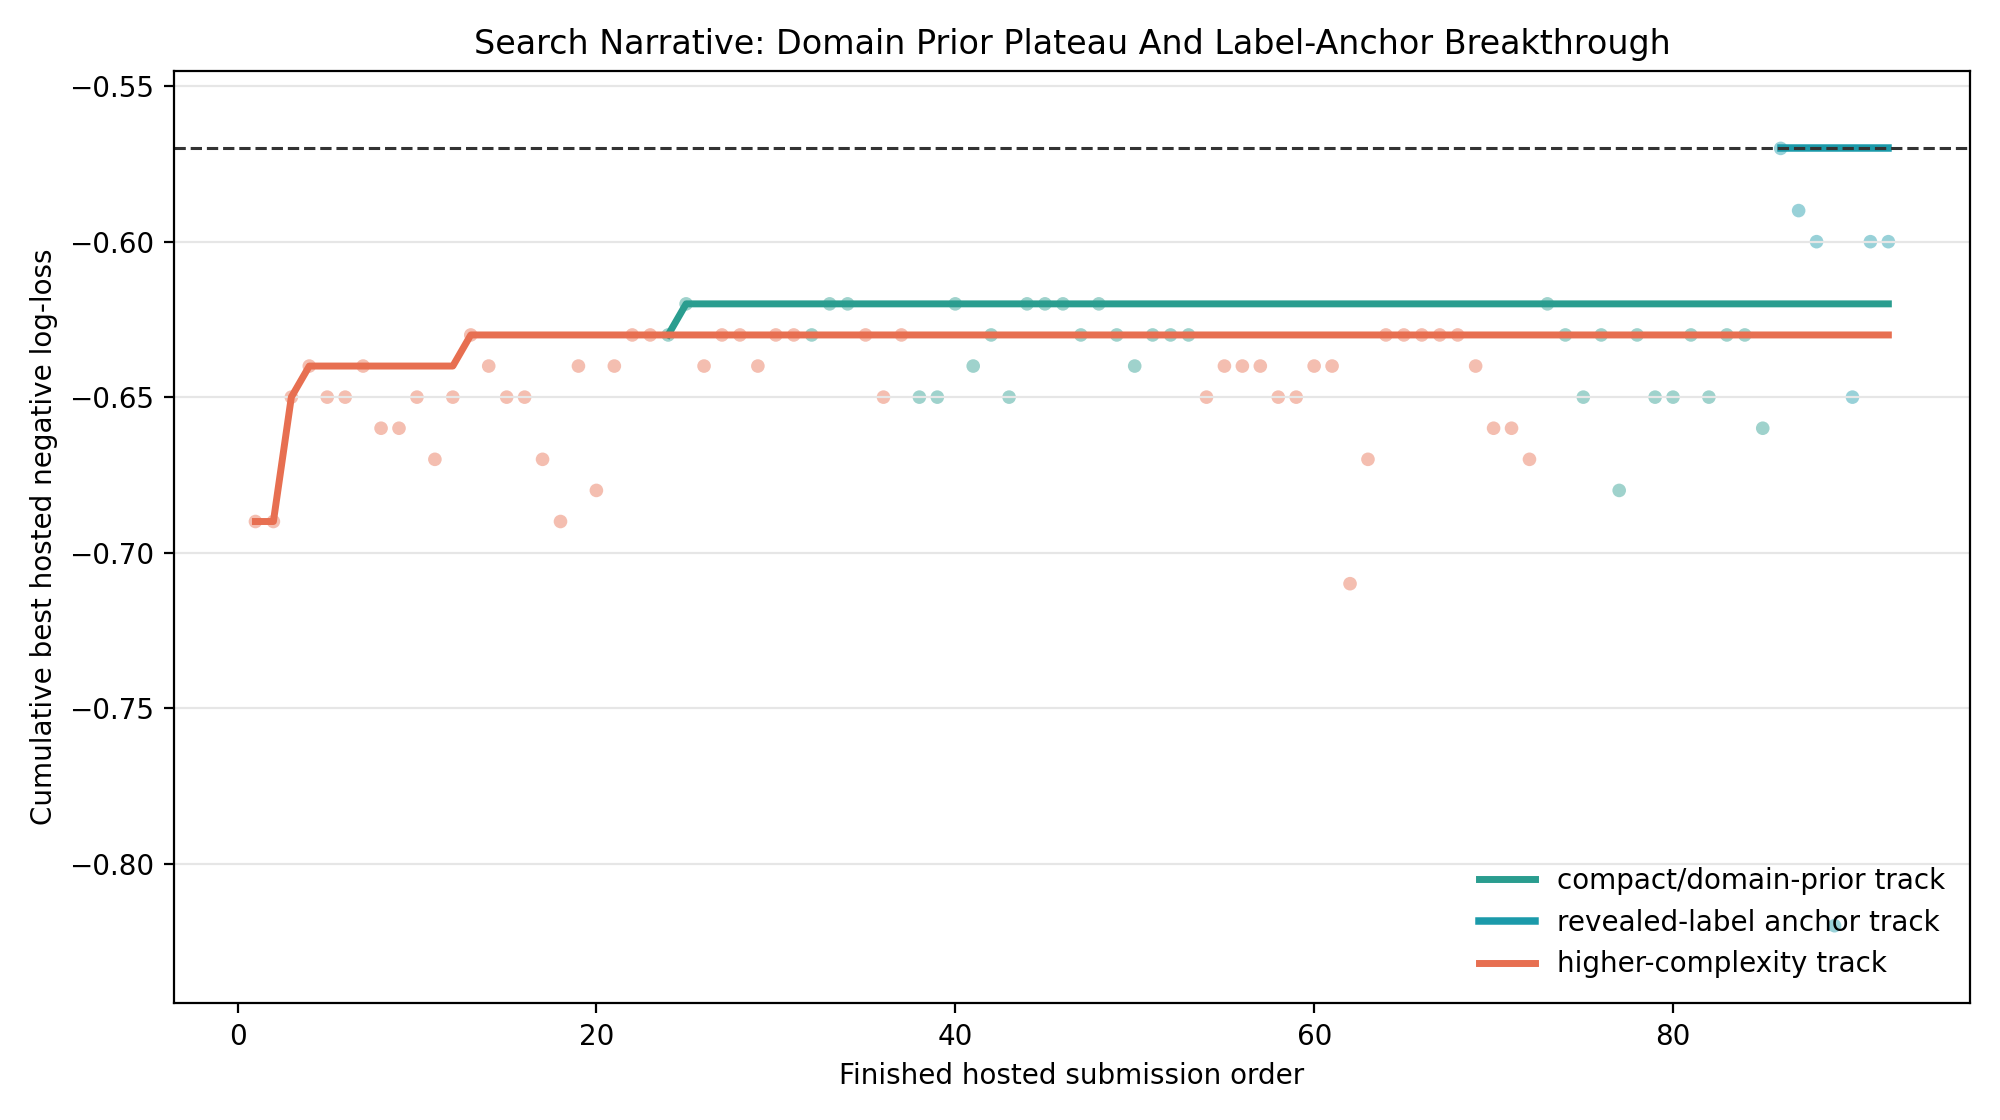
\includegraphics[width=\linewidth]{figures/search_narrative.png}
  \caption{Cumulative best score for compact/domain-prior candidates, higher-complexity candidates, and revealed-label anchor candidates.}
  \label{fig:narrative}
\end{figure}

\section{Why High Local AUC Did Not Transfer}
The hosted evidence shows that public-slice AUC was not reliable promotion evidence for this competition.

\paragraph{Validation overlap was too permissive.}
Public-slice probes sampled from the same public matrix used to build many artifacts, preserving subject, benchmark, condition, and sometimes item overlap. Exact item memory had high row-holdout coverage but zero benchmark-holdout item coverage.

\paragraph{AUC rewarded ranking rather than calibration.}
AUC-heavy models used wide probability spreads. That can rank familiar rows well while worsening log-loss on shifted hidden families. The strict benchmark-holdout audit already showed weak transfer, with weighted log-loss 0.729388 and weighted AUC 0.537691.

\paragraph{Hidden benchmark families changed the base-rate problem.}
Models could learn that a public benchmark was easy or hard, but that did not identify the hidden benchmark family's base rate. The compact domain prior was robust because it stayed broad; the anchor improved further because it estimated the hidden-run base rate directly from revealed labels.

\section{Final Selected Method}
The selected method is \texttt{submission\_anchor\_fam\_b60\_debias.zip}. Its runtime formula is:
\[
  p_{s,i}
  =
  \sigma\left(
    \tilde\ell_{g^*(i)}-\beta\bar o_L+\beta o_{s,f(i)}
  \right).
\]
The term \(\tilde\ell_{g^*(i)}\) is the shrunk hidden-run base-rate logit from random revealed labels, \(o_{s,f(i)}\) is a family-relative subject offset, and \(\bar o_L\) debiases the revealed sample for subject composition. The ZIP contains only \path{model.py} and \path{artifacts/domain_prior.json}. It has no \path{labeling.py}, no exact item-memory table, no tree model, and no forecast ensemble.

This method achieved the competition target of log-loss below 0.60. It replaced \path{submission_domain_live_mid600.zip} as the final selection because the updated hosted evidence gave it score -0.57 and competition-reported AUC-ROC 0.73.

\section{Lessons Learned And Future Work}
Hosted negative log-loss must remain the objective. Public-proxy AUC can diagnose ranking signal, but it should not promote a submission unless cold benchmark-family log-loss and calibration also improve.

The most useful future work is better hidden-run base-rate estimation. That means more robust grouping keys for revealed labels, better small-\(K\) variance control, and subject-family offsets trained without benchmark-family leakage. Active labeling should remain disabled unless it beats platform-random labels while preserving an unbiased category base-rate estimate.

\section{Clean Publication Repository}
The clean publication artifact is organized as \path{aims-competition} and published at \url{https://github.com/BlakeMasters/aims-competition}. It contains the final uploadable ZIP, extracted final submission source, archived alternate submission ZIPs under \path{unused_submissions}, this report as PDF and LaTeX source, generated figures and tables, hosted-results files, minimal validation tools, and tiny sample files for smoke testing. It intentionally excludes raw benchmark downloads, validation extraction folders, virtual environments, Python caches, agent instructions, documentation folders, and iterative working artifacts.

\section{Reproducibility}
The hosted-results tables and figures were regenerated from \texttt{eval\_finals.txt}. The parser found 94 hosted rows and 92 finished scored rows. The best rounded hosted score was -0.57, tied by 1 finished rows in the cleaned hosted result table. The derived CSV files under \texttt{report/tables/} provide the exact counts used in Table~\ref{tab:family-summary}.

\bibliographystyle{plain}
\bibliography{references}

\end{document}
